\section{ Reagents: expressing and composing fine-grained concurrency \cite{reagent2012}}

\subsection{Motivation}
Amidst a sea of non-blocking progress guarantees, wait-free algorithms offer the strongest promise, every thread completes in a bounded number of steps regardless of interference, but are notoriously difficult to design and reason about. At the other end, obstruction-free algorithms guarantee progress only in the absence of contention, making them easier to construct but weaker in practice. Lock-free data structures occupy the practical sweet spot: they ensure system-wide progress (at least one thread completes) while remaining implementable and scalable. Modern libraries such as \texttt{java.util.concurrent} provide highly optimized lock-free stacks, queues, and maps, yet these structures are not \emph{composable}. For instance, performing \texttt{x = A.pop(); B.push(x);} is not atomic; between the two calls, another thread may observe inconsistent intermediate state. Extending the library with ad hoc methods like \texttt{popAndPush} leads to API explosion and violates a key abstraction principle: libraries should expose composable building blocks, not bespoke combinations. In traditional lock-free programming, the developer must explicitly orchestrate CAS loops, retries, and memory interactions, thereby controlling the low-level protocol. Reagents address this gap by introducing a new execution model. A reagent, written $\texttt{Reagent}[A,B]$, is a \emph{description} of a concurrent atomic interaction: given input $A$, it performs coordinated memory updates and synchronization to produce $B$, while abstracting away CAS retries, transient failures, and commit protocols. By treating atomic operations as first-class composable values, reagents allow developers to declaratively specify interactions while the runtime enforces lock-free coordination. In doing so, they reconcile scalability with composability, avoiding global locks, heavyweight transactional memory, and abstraction-breaking APIs.

\subsection{Proposed Solution}

Reagents attempt to reconcile two historically distinct models of concurrency.
The first model is the \emph{shared-state paradigm}, in which threads coordinate
by reading and writing shared memory locations using atomic primitives such as
compare-and-swap (CAS). In this setting, correctness depends on carefully
maintaining invariants over mutable state, and progress is achieved through
retry loops that repeatedly attempt atomic updates. Lock-free stacks and queues
are canonical examples of this approach.

The second model is the \emph{message-passing paradigm}, in which threads do not
interact by sharing memory directly but instead exchange values over channels.
Synchronization is achieved through structured communication rather than
low-level atomic instructions. This approach emphasizes clarity and composability,
as communication events themselves become the unit of coordination.

Reagents unify these traditions by treating atomic memory updates as
first-class synchronization events. In effect, they allow CAS-based
interactions from the shared-state world to be composed in a manner similar
to communication events in the message-passing world.

\begin{figure}[t]
\begin{lstlisting}[language=Go,
  basicstyle=\small\ttfamily,
  breaklines=true,
  columns=flexible]
ch := make(chan int)
go func() {
  ch <- 10  // send
}()
x := <-ch  // receive
\end{lstlisting}
\caption{Basic channel creation and rendezvous in Go.}
\label{fig:go-basic}
\end{figure}

\noindent
The send operation (\autoref{fig:go-basic}) \lstinline{ch <- 10} blocks until
another goroutine performs a corresponding receive \lstinline{x := <-ch}.
This rendezvous ensures that communication and synchronization occur
simultaneously, without exposing shared-memory races. Go also provides
selective communication through the \lstinline{select} statement:

\begin{figure}[t]
\begin{lstlisting}[language=Go,
  basicstyle=\small\ttfamily,
  breaklines=true,
  columns=flexible]
select {
case x := <-ch1:
  fmt.Println("Received from ch1:", x)
case y := <-ch2:
  fmt.Println("Received from ch2:", y)
default:
  fmt.Println("No channel ready")
}
\end{lstlisting}
\caption{Selective communication using \lstinline{select} in Go.}
\label{fig:go-select}
\end{figure}

The \lstinline{select} statement waits until one of the communication operations is enabled. If multiple cases are ready, one is chosen non-deterministically. If none are ready and a \lstinline{default} clause is present, execution proceeds with that branch; otherwise, the goroutine blocks. This construct exemplifies \emph{selective communication}, where the runtime determines which interaction can proceed. The same conceptual mechanism appears in Concurrent ML via the \lstinline{choose} combinator, where synchronization events are treated as first-class values and composed algebraically.


\subsection{Algebra of Reagents}
Reagents introduce a small but expressive algebra for composing concurrent atomic interactions. At its core are three combinators: sequencing ($r_1 \;\;\; r_2$), parallel conjunction ($r_1 \;\ast\; r_2$), and choice ($r_1 \;|\; r_2$). Sequencing composes two reagents transactionally, ensuring that the effect of $r_2$ logically follows $r_1$ within a single atomic interaction. Parallel conjunction requires that both $r_1$ and $r_2$ be enabled and commit together, forming a coordinated atomic update across multiple memory locations. Choice allows the system to attempt multiple interactions and commit whichever becomes enabled first, reminiscent of selective communication. Unlike Software Transactional Memory (STM), where an \texttt{atomic} block tracks all reads and writes within its scope and validates them during commit, reagents expose only explicitly declared atomic updates; speculative reads remain invisible and do not participate in global validation. Composition therefore occurs at well-defined commit boundaries rather than at the level of arbitrary memory accesses. For example, composing $\texttt{pop}(A) \;\;\; \texttt{push}(B)$ yields an atomic transfer between two lock-free stacks without introducing a global transaction that tracks every intermediate read. Similarly, $r_1 \;|\; r_2$ allows a program to proceed with whichever operation becomes feasible first, and $r_1 \;\ast\; r_2$ coordinates multiple atomic updates as a single interaction. In this way, reagents provide algebraic composition of lock-free operations while avoiding the heavyweight bookkeeping characteristic of STM.


\subsection{Implementation Overview}

Reagents execute via a conceptually two-phase protocol~\cite{turon2012thesis}.
When a reagent is invoked (via the \texttt{!} method), it attempts to
\emph{react}. Reaction consists of (1) a \emph{collection phase}, during which
the runtime builds up a \texttt{Reaction} object containing the atomic updates
(e.g., CAS operations), messages, and post-commit actions; and (2) a
\emph{commit phase}, during which the collected updates are atomically applied.

A failure during the first phase (i.e., failure to build the desired reaction)
is classified as a \emph{permanent failure}. This corresponds to logical
impossibility under current conditions (e.g., popping from an empty stack with
no alternative branch). Retrying would not help; the reagent must block until
external state changes. By contrast, a failure during the commit phase is a
\emph{transient failure}: the reaction was valid, but interference from another
thread prevented atomic commitment. In this case, the system retries.

Internally, outcomes are represented as:

\begin{figure}[t]
\centering
\begin{minipage}{0.9\linewidth}
\begin{verbatim}
type 'a result =
  | Block        (* permanent failure *)
  | Retry        (* transient failure *)
  | Done of 'a   (* successful commit *)

type ('a,'b) t = {
  try_react      : 'a -> reaction -> offer option -> 'b result;
  compose        : 'r. ('b,'r) t -> ('a,'r) t;
  always_commits : bool;
  may_sync       : bool;
}
\end{verbatim}
\end{minipage}
\caption{Core internal representation of reagents (adapted from~\cite{turon2012thesis}).}
\label{fig:reagent-core}
\end{figure}

The \texttt{try\_react} method attempts to extend the current reaction; it may
complete (\texttt{Done}), block permanently (\texttt{Block}), or signal
interference (\texttt{Retry}). The \texttt{compose} field implements the
algebraic combinators, while \texttt{always\_commits} and \texttt{may\_sync}
provide static hints for optimization.

Reagents are implemented in continuation-passing style (CPS). Rather than
represent sequencing as a separate structural node, each reagent carries its
own continuation—a reagent describing the remainder of the computation. The
initial continuation is \texttt{Commit}, which transitions from building a
\texttt{Reaction} to actually committing it. The sequencing combinator
therefore merely wires continuations together.

CPS can be illustrated in Racket:

\begin{figure}[t]
\centering
\begin{minipage}{0.9\linewidth}
\begin{verbatim}
(define (safe-div x y k)
  (if (= y 0)
      (k 'error)
      (k (/ x y))))
\end{verbatim}
\caption{A simple continuation-passing style example.}
\label{fig:cps}
\end{minipage}
\end{figure}

Here, instead of returning a value, \texttt{safe-div} invokes continuation
\texttt{k}. Control flow is made explicit. Similarly, in reagents,
continuations encode ``what to do next'' after a reaction step, enabling
backtracking choice and message passing without additional runtime constructs.

The commit phase requires atomically applying multiple CAS operations when a
reaction spans multiple locations. This is implemented as a $k$-CAS protocol.
When hardware transactional memory (HTM) is available, it can accelerate this
phase; otherwise, a descriptor-based software multi-word CAS is used. In the
common case where a reagent performs only a single visible CAS, the runtime
optimizes by executing it directly, avoiding the overhead of constructing a
full \texttt{Reaction} object.

Overall, the internal structure can be summarized as:

\begin{verbatim}
build reaction  →  Block | Retry | proceed
proceed         →  k-CAS commit
commit result   →  Done | Retry
\end{verbatim}

Collection determines feasibility; commit ensures atomicity; CPS enables
compositional control flow. Together, these mechanisms allow reagents to
support composable lock-free interactions without global locking or
heavyweight STM.

\begin{figure}[t]
\centering
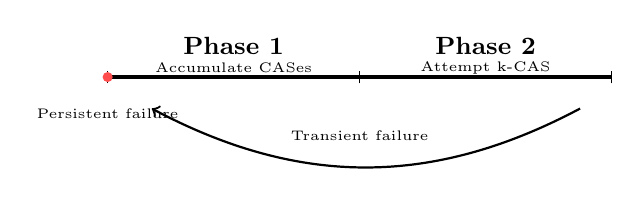
\begin{tikzpicture}[scale=0.8]
  % Main timeline
  \draw[ultra thick] (0.5,0) -- (8.5,0);

  % Tick marks
  \foreach \x in {0.5, 4.5, 8.5} {
    \draw (\x, -0.1) -- (\x, 0.1);
  }

  % Phase labels (positioned above timeline)
  \node[align=center, font=\bfseries\small] at (2.5, 0.5) {Phase 1};
  \node[align=center, font=\tiny] at (2.5, 0.15) {Accumulate CASes};

  \node[align=center, font=\bfseries\small] at (6.5, 0.5) {Phase 2};
  \node[align=center, font=\tiny] at (6.5, 0.15) {Attempt k-CAS};

  % Persistent failure: just a dot on timeline
  \fill[red!70] (0.5, 0) circle (0.08);
  \node[anchor=north, font=\tiny] at (0.5, -0.35) {Persistent failure};

  % Transient failure arc (below)
  \draw[thick, <-, bend right=28] (1.2, -0.5) to (8, -0.5);
  \node[anchor=north, font=\tiny] at (4.5, -0.7) {Transient failure};
\end{tikzpicture}
\caption{Two-phase CAS protocol: persistent failures at start prevent completion;
transient failures allow retry.}
\label{fig:cas-phases}
\end{figure}


\subsection{Conclusion}
Reagents suggest a transactional abstraction for lock-free data structures with explicit commit boundaries. Such structure may significantly simplify reasoning about linearization points and compositional correctness. Developing a formal operational semantics could therefore provide a foundation for automated linearizability verification in the presence of both shared-state and message-passing interactions.
